\chapter{Framework}\label{chapter:framework}
% TODO(style): deviates from template -- HAOS, BG-AILS, the DRI loop, and
% SC/SP are introduced by manual spelling below rather than through
% \gls{}/\newacronym, matching every other use of these terms in this
% chapter (Sections 4.1-4.6, written before this intro). Flagged per
% STYLE.md \S8 rather than silently rewritten; a future pass could add
% glossary entries for all four and switch the whole chapter over at once.

This chapter presents DRISPI, the framework this thesis develops for the \gls{cvrp} at very-large scale (Section~\ref{sec:lit-problem}). DRISPI repeatedly executes a decompose-route-improve (DRI) loop. Each iteration first partitions the customer set into smaller subclusters and solves one routing subproblem per subcluster with an existing monolithic solver, then concatenates the resulting routes and revises them near the subcluster boundaries with a dedicated improvement stage, boundary-guided adaptive iterated local search (BG-AILS). Hierarchical adaptive operator selection (HAOS) draws the decomposition and routing configuration for every iteration from a set of weighted alternatives and updates those weights from the outcomes it observes, rather than fixing one configuration for the whole run. Every route the DRI loop produces enters a persistent route pool; at scheduled intervals, DRISPI steps back from the current incumbent and recombines the pool through a set covering or set partitioning (SC/SP) model, followed by one further improvement pass. The loop continues until a wall-clock time limit or a run of iterations without improvement is reached.

Figure~\ref{fig:dri-overview} shows the resulting control flow for one instance. HAOS (Section~\ref{sec:fra-haos}) draws one configuration per iteration; decomposition (Section~\ref{sec:fra-decomposition}) partitions the customer set into $k$ subclusters under that configuration; routing (Section~\ref{sec:fra-routing}) solves each subcluster independently and concatenates the routes; BG-AILS (Section~\ref{sec:fra-bg-ails}) revises the routes near the subcluster boundaries. Both the routing stage and BG-AILS add their routes to the route pool, and either can become the new incumbent if it improves on the current one. At scheduled intervals, the same iteration also runs set covering or set partitioning (Section~\ref{sec:fra-sp}) over the pool accumulated so far, followed by one further improvement pass (Section~\ref{sec:fra-improve}) whose output feeds the pool again and can likewise become the new incumbent; on every other iteration, this pair of stages is skipped. The loop then either returns to a fresh HAOS draw or stops. Figure~\ref{fig:dri-overview} shows this control flow as one sequential loop; Section~\ref{sec:fra-pipeline} shows how DRISPI executes it with several stages running in parallel across iterations instead.

\begin{figure}[H]
\centering
\begin{tikzpicture}[
    x=1cm, y=1cm,
    startstop/.style={ellipse, draw, thick, minimum width=2.1cm, minimum height=0.9cm, align=center, fill=gray!12},
    process/.style={rectangle, draw, thick, rounded corners=2pt, minimum width=4.4cm, minimum height=1.05cm, align=center, fill=blue!6},
    decision/.style={diamond, draw, thick, aspect=2.4, inner sep=1pt, align=center, fill=orange!8, text width=2.7cm},
    poolbox/.style={rectangle, draw, thick, dashed, minimum width=2.5cm, minimum height=10.2cm, align=center, fill=gray!5},
    arr/.style={-{Latex[length=2.2mm,width=1.6mm]}, thick},
    lbl/.style={font=\footnotesize},
    ]

   
    \node[startstop] (start) at (3,21.0) {Start};
    \node[process]   (haos)    at (3,19.1) {HAOS draws a configuration};
    \node[process]   (decomp)  at (3,17.4) {Decomposition into $k$ subclusters};
    \node[process]   (routing) at (3,15.7) {Routing (parallel, then concatenated)};
    \node[process]   (bgails)  at (3,14.0) {BG-AILS};
    \node[decision]  (dec1)    at (3,11.7) {SC/SP scheduled?};
    \node[process]   (scsp)    at (3,9.2)  {SC/SP};
    \node[process]   (improve) at (3,7.5)  {Improvement (AILS-II)};
    \node[decision]  (dec2)    at (3,4.6)  {Stopping criterion met?};
    \node[startstop] (end)     at (3,2.4)  {End};
    \node[poolbox]   (pool)    at (8.7,12.4) {};
    \node[lbl] at (8.7,16.6) {Route Pool};

    \draw[arr] (start) -- (haos);
    \draw[arr] (haos) -- (decomp);
    \draw[arr] (decomp) -- (routing);
    \draw[arr] (routing) -- (bgails);
    \draw[arr] (bgails) -- (dec1);
    \draw[arr] (dec1) -- node[lbl,left] {yes} (scsp);
    \draw[arr] (scsp) -- (improve);
    \draw[arr] (improve) -- (6.2,6.1) -- (dec2);
    \draw[arr] (dec1.east) -- node[lbl,above] {no} (10.6,11.7) -- (10.6,6.1) -- (dec2.east);
    \draw[arr] (dec2) -- node[lbl,left] {yes} (end);
    \draw[arr] (dec2.west) -- node[lbl,above,pos=0.75] {no} (-1.6,4.6) -- (-1.6,19.1) -- (haos.west);
    \node[lbl] at (-1.6,12.0) {\rotatebox{90}{next iteration}};

    \draw[arr] (routing.east) -- node[lbl,above] {feed} (7.45,15.7);
    \draw[arr] (bgails.east) -- node[lbl,above] {feed} (7.45,14.0);
    \draw[arr] (improve.east) -- node[lbl,above] {feed} (7.45,7.5);
    \draw[arr] (7.45,9.2) -- node[lbl,above] {read} (scsp.east);
\end{tikzpicture}
\caption{Sequential control flow of one DRISPI run: the DRI loop, the route pool, and periodic SC/SP recombination.}
\label{fig:dri-overview}
\end{figure}

The remaining sections address one stage each, in the order Figure~\ref{fig:dri-overview} shows: Section~\ref{sec:fra-haos} on HAOS, Section~\ref{sec:fra-decomposition} on decomposition, Section~\ref{sec:fra-routing} on routing, Section~\ref{sec:fra-bg-ails} on BG-AILS, Section~\ref{sec:fra-sp} on the route pool and SC/SP, and Section~\ref{sec:fra-improve} on the post-SC/SP improvement pass. Section~\ref{sec:fra-pipeline} closes the chapter by assembling these stages into the parallelized pipeline DRISPI actually runs, together with the pseudocode for its control loop.

\section{Hierarchical Adaptive Operator Selection}\label{sec:fra-haos}
Ideally, a heuristic would always be tuned to no more than one specific problem instance. That would promise both, an effective and efficient approach configured to exploit that instance's size, spatial and demand distributions, and fleet capacity. Recent benchmark sets however have deliberately combined a wide range of these characteristics to test whether performance transfers across instance structures \citep{uchoaNewBenchmarkInstances2017,queirogaXLInstancesCapacitated2026}. That is why finding and selecting a tailored configuration for every instance requires a costly tuning campaign. That is why most benchmarks are compromising on one fixed configuration for the entire problem set. This framework aims to forego this compromise through Hierarchical Adaptive Operator Selection (HAOS), an approach to adapt DRISPI's configuration while solving the problem instead.

The principal methodological inspiration is adaptive large neighborhood search. Competing destroy and repair operators receive weights based on observed performance and are selected by roulette wheel \citep{ropkeAdaptiveLargeNeighborhood2006}. The same adaptive layer has been applied across five vehicle routing variants \citep{pisingerGeneralHeuristicVehicle2007}. HAOS adopts this principle but moves the adaptive choice outside a single local search. It instead controls the decomposition granularity, the representation and method used for clustering, the demand contribution cluster formation, as well as the subsolver. The adaptation is online because rewards update the weights while the current instance is being solved. The weights of each operator summarize observed performance on that instance. The Convergence to a globally optimal configuration is neither required nor guaranteed.

The operator choices can also be interpreted as arms of a multi-armed bandit. After an arm is drawn, the search observes a reward but does not know what the unselected arms would have produced. This analogy connects HAOS to the exploration--exploitation problem \citep{auerFinitetimeAnalysisMultiarmed2002} and to bandit-based adaptive operator selection \citep{fialhoAnalyzingBanditbasedAdaptive2010}. However, HAOS does not implement a confidence-bound policy, an explicit exploration bonus, or a separate exploratory action. Its roulette probabilities follow the current weights directly. Stochastic sampling leaves every positive-weight option selectable, while the probability-floor transformation described below raises normalized shares that become sufficiently small.
% not entirely happy with this paragraph. Foreshadowing usually indicates poor structure. Evaluate later.

% Maybe write the Levels in bold? Or use a different way to explain them clearer. Like an indented enumeration
At the beginning of every DRI iteration HAOS draws one configuration across five levels. Level one selects the number of subclusters $k$ from a scale-adaptive domain. Its base values are clipped to the instance's minimum feasible fleet size and extended geometrically for larger instances. The number of arms is capped at ten to allow for convergence to occur within a reasonable wallclock time. Level two selects the demand weight $\lambda_q$ from six evenly spaced values between zero and one; this value controls how strongly differences in customer demand influence the decomposition. Level three selects whether customers are clustered directly (the vertex-based paradigm) or through the routes of the current incumbent solution (the route-based paradigm). Level four selects a clustering method from the wheel associated with the chosen paradigm, with five vertex-based and three route-based methods in the deployed configuration. This conditional fourth level makes the selection hierarchical since the selection on level four directly depends on level three. Level five selects one of four routing solvers and applies it to every subcluster generated during the iteration. The first four levels therefore configure decomposition, and the fifth configures subproblem routing.

Two feasibility adjustments apply before the configuration is used; Algorithm~\ref{alg:haos} gives the draw and update in full. Route-based clustering requires an incumbent solution. Without one, HAOS uses the vertex-based paradigm and redraws the method from the vertex wheel; these applied choices receive the subsequent credit. If $k$ exceeds the number of incumbent routes under route-based clustering, the applied $k$ is clipped to the route count. The immediate update retains the index of the $k$ arm originally drawn, while route tags record the configuration that was applied. Each iteration is logged with the complete operator selection and the product of the five selected probabilities, which reports the joint probability of the realized configuration under the current wheels.

HAOS maintains six roulette wheels for the five levels, because of the conditional clustering method level. Each wheel tracks one weight per option. A reward $r$ adds to the weight of every arm selected for the credited configuration. Once per iteration, every weight is also multiplied by a common decay factor. This uniform decay is the only temporal mechanism in the weights. Both operations retain the starting weight as a lower bound:
\begin{align}
w_i &\leftarrow \max(w_i + r,\ w_0), \label{eq:haos-update}\\
w_i &\leftarrow \max(\gamma w_i,\ w_0), \qquad \gamma = 0.95 \text{ by default,} \label{eq:haos-decay}
\end{align}
with every wheel starting from the same weight $w_0~=~10.0$.  Before an arm is drawn, HAOS first computes its normalized weight $\hat{p}_i = w_i / \sum_l w_l$. A level-specific floor is applied to these values, followed by renormalization:
\begin{equation}
p_i = \frac{\max(\hat{p}_i,\ p_{\mathrm{min}})}{\sum_j \max(\hat{p}_j,\ p_{\mathrm{min}})}.
\label{eq:haos-probability}
\end{equation}
The floor parameter is the minimum probability any weight of any wheel can decay to. For the five levels, the floors are 0.025 for $k$, 0.05 for $\lambda_q$, the clustering methods, and the solver, and 0.10 for the paradigm respectively. Because Equation~\ref{eq:haos-probability} renormalizes after flooring, these values are nominal pre-normalization floors rather than strict lower bounds on the final probabilities. HAOS retains three elements of the adaptive layer proposed by \citet{ropkeAdaptiveLargeNeighborhood2006} and used for general vehicle routing by \citet{pisingerGeneralHeuristicVehicle2007}: initially equal weights, quality-dependent scores, and roulette selection proportional to the resulting weights. Its additive reward, global decay, and six-wheel hierarchy are novelties introduced for DRISPI\@.

HAOS adapts its weights by receiving rewards from later stages of the current or following iterations. First, there is an immediate channel for results produced directly by the current DRI iteration and a deferred channel for routes that prove useful during later pool recombination. Table~\ref{tab:haos-rewards} gives the deployed reward values. Both channels compare a candidate with the incumbent best cost and the previous iteration's cost, but the deferred scores are smaller because several earlier configurations can contribute routes to the same recombined solution.

\begin{table}[H]
\centering
\caption{Default Immediate and Deferred HAOS Rewards.}
\label{tab:haos-rewards}
\begin{tabular}{lcc}
\toprule
Outcome & Immediate & Deferred \\
\midrule
New incumbent best & 10.0 & 7.0 \\
Improvement over previous iteration only & 4.0 & 3.0 \\
No improvement & 1.0 & 0.0 \\
No solution & 0.0 & 0.0 \\
\bottomrule
\end{tabular}
\end{table}

The immediate channel scores two candidates: the solution obtained after decomposition and subproblem routing, and the solution obtained after BG-AILS. Both rewards are credited to the same five-level configuration drawn for that iteration and therefore accumulate. Each selected arm receives the full reward. By doing so, HAOS learns from the performance of the complete configuration but does not isolate the contribution of one level or model interactions between levels.

\begin{algorithm}[H]
\DontPrintSemicolon
\LinesNumbered
\SetKwInOut{Input}{Input}
\SetKwInOut{Output}{Output}
\Input{wheels $W_1, W_2, W_3, W_{4v}, W_{4r}, W_5$; incumbent route count $m_{\mathrm{inc}}$; floors $p_{\min}^{(1)}, \ldots, p_{\min}^{(5)}$; decay $\gamma$; base weight $w_0$}
\Output{applied configuration $(k, \lambda_q, \mathrm{paradigm}, \mathrm{method}, \mathrm{solver})$}
draw $k, \lambda_q, \mathrm{paradigm}, \mathrm{solver}$ from $W_1, W_2, W_3, W_5$ \tcp*{Eq.~\ref{eq:haos-probability}}
\eIf{paradigm $=$ route}{draw method from $W_{4r}$}{draw method from $W_{4v}$}
credited $\gets (k, \lambda_q, \mathrm{paradigm}, \mathrm{method}, \mathrm{solver})$ \tcp*{as drawn}
\If{paradigm $=$ route and $m_{\mathrm{inc}}$ undefined}{
  paradigm $\gets$ vertex; redraw method from $W_{4v}$; overwrite it in credited\;
}
$k_{\mathrm{applied}} \gets k$\;
\If{paradigm $=$ route and $k > m_{\mathrm{inc}}$}{
  $k_{\mathrm{applied}} \gets m_{\mathrm{inc}}$ \tcp*{credited keeps the drawn $k$}
}
run decomposition and routing under $(k_{\mathrm{applied}}, \lambda_q, \mathrm{paradigm}, \mathrm{method}, \mathrm{solver})$\;
tag every produced route with this applied configuration\;
\ForEach{candidate $\in$ (decompose-route solution, BG-AILS solution)}{
  $r \gets$ reward of candidate from Table~\ref{tab:haos-rewards}\;
  \ForEach{arm $i \in$ credited}{
    $w_i \gets \max(w_i + r,\ w_0)$ \tcp*{Eq.~\ref{eq:haos-update}}
  }
}
\ForEach{wheel $W \in \{W_1, W_2, W_3, W_{4v}, W_{4r}, W_5\}$, arm $i \in W$}{
  $w_i \gets \max(\gamma w_i,\ w_0)$ \tcp*{Eq.~\ref{eq:haos-decay}}
}
\caption{HAOS: five-level draw and weight update for one DRI iteration}
\label{alg:haos}
\end{algorithm}

Lines 10-11 are the feasibility clipping that matters for correctness: when route-based clustering draws a $k$ larger than the incumbent route count, only $k_{\mathrm{applied}}$ on line 11 changes; the credited configuration fixed on line 6 keeps the originally drawn $k$-arm. Lines 14-17 are the reward credit itself: both the decompose-route candidate and the BG-AILS candidate (line 14) add their reward (line 15) to every arm in credited (lines 16-17), so a single iteration's two immediate rewards accumulate on the same five arms regardless of whether $k$ had to be clipped on line 11. This is why clipping does not by itself distort the immediate update: the arm being rewarded is the one HAOS drew on line 6, not the one the pipeline used after line 11.

The deferred channel is evaluated after SC/SP has selected routes from the pool and the resulting solution has received its unrestricted improvement pass. Every stored route carries a tag containing the complete configuration under which it was generated. The deferred reward is credited once to every distinct tag among the routes selected by SC/SP, even if those tags originate from much earlier iterations. Routes created only during the unrestricted improvement pass are excluded because no HAOS selection produced them. Deferred attribution is necessary because the usefulness of one stored route may become visible only when it is combined with routes generated later.

During the first 10 iterations, HAOS performs the same five-level draw but suppresses both reward updates and decay. All weights therefore remain equal, making every option uniform within the wheel from which it is eligible to be drawn. This warm-up period lets the first incumbent and an initial route pool form before early outcomes influence later probabilities. Learning begins with iteration 10, after which the immediate and deferred updates follow the same weight system.

\section{Decomposition}\label{sec:fra-decomposition}
% NOTE(citations-added-this-pass, not yet verified by the author): the following
% keys are new to bibliography/literature.bib as of this draft and should be
% checked for relevance and correctness before the next build:
% gillettHeuristicAlgorithmVehicleDispatch1974, fisherGeneralizedAssignmentHeuristic1981,
% kaufmanFindingGroupsData1990, bezdekFCMFuzzyCmeans1984,
% macqueenMethodsClassificationAnalysis1967, kerscherDecomposerouteimproveFrameworkSolving2025,
% kerscherSolvingHeterogeneousVehicle, santiniDecompositionStrategiesVehicle2023.

% I believe this section can be made a bit longer. We can definitely reference the literature review section on decomposition and clustering approaches more often once it is written. Also, maybe go into more depth on how each clustering method works (with sources)

% part of this paragraph can be moved into the introduction 4.0 I think
The decomposition layer runs at the beginning of every iteration in the DRI loop, adapting the decompose-route-improve terminology of \citet{kerscherDecomposerouteimproveFrameworkSolving2025}, who propose the framework for large-scale vehicle routing problems with time windows that this work extends to the \gls{cvrp} at very-large scale in a fully parallelized, self-tuning setting. HAOS (Section~\ref{sec:fra-haos}) controls this stage through four levels, redrawn at every iteration: first the number of subclusters k; second the clustering paradigm, either vertex-based, which partitions the customers directly, or route-based, which partitions the routes of the current incumbent solution and propagates the resulting labels to their customers; third the clustering method used within that paradigm; and fourth the demand weight $\lambda_q$ of the dissimilarity metric utilized a subset of clustering approaches. Additionally, a fifth quantity that also feeds the metric, the angular offset $\phi$, is drawn uniformly from $[0, 2\pi)$ at every iteration independently of HAOS. $\phi$ ensures that the wraparound point described below does not stay fixed across iterations.

For the decomposition, we form a dissimilarity metric that combines three terms for every pair of customers i and j with coordinates $(x_i, y_i)$ and $(x_j, y_j)$ and demands $q_i$ and $q_j$: their Euclidean distance, an angular term, and a demand term,
\begin{equation}
d_{ij} = \sqrt{(x_i - x_j)^2 + (y_i - y_j)^2 + \lambda_\theta \, \Delta\theta_{ij}^2\,} \left(1 + \lambda_q \frac{|q_i - q_j|}{Q}\right).
\label{eq:decomp-dissimilarity}
\end{equation}
$\Delta\theta_{ij}$ is the shortest angular distance between customer i's and customer j's polar angle around the depot, computed with the offset $\phi$ introduced above. $\lambda_\theta$ scales the angular term to the average coordinate magnitude of the instance, so that neither term dominates across instances of different spatial extent. $\phi$ shifts where the $\Delta\theta_{ij}$ wraparound at $2\pi$ falls. The demand factor applies the multi-feature dissimilarity metric of \citet{kerscherDecomposerouteimproveFrameworkSolving2025}, who combine spatial, temporal, and demand features, here to a setting without time windows, utilizing only the demand ratio $\lambda_q |q_i - q_j| / Q$ remains alongside spatial features.

\begin{table}[H]
\centering
\caption{Inputs Used By Each Decomposition Method.}
\label{tab:decomp-methods}
\begin{tabular}{llccc}
\toprule
Method & Paradigm & Input & Angular & Demand \\
\midrule
K-Means & vertex & raw coordinates & -- & -- \\
Fuzzy C-Means & vertex & raw coordinates & -- & -- \\
K-Medoids & vertex & dissimilarity matrix & \checkmark & \checkmark \\
Agglomerative (Average) & vertex & dissimilarity matrix & \checkmark & \checkmark \\
Agglomerative (Complete) & vertex & dissimilarity matrix & \checkmark & \checkmark \\
K-Means & route & route centroids & -- & -- \\
Agglomerative (Average) & route & route centroids & -- & -- \\
Agglomerative (Complete) & route & route centroids & -- & -- \\
\bottomrule
\end{tabular}
\end{table}

Both clustering paradigms trace back to the classic cluster-first, route-second scheme for capacitated routing \citep{gillettHeuristicAlgorithmVehicleDispatch1974, fisherGeneralizedAssignmentHeuristic1981}, reviewed with route-first cluster-second and with vertex-based versus route-based clustering in Section~\ref{sec:lit-decomposition}. Vertex-based clustering partitions the customers directly and offers five methods (Table~\ref{tab:decomp-methods}). K-Means \citep{macqueenMethodsClassificationAnalysis1967} and Fuzzy C-Means \citep{bezdekFCMFuzzyCmeans1984} cluster on raw two-dimensional coordinates, Fuzzy C-Means hardened to a partition by assigning each customer to its highest-membership cluster. The remaining methods K-Medoids, partitioning around medoids \citep{kaufmanFindingGroupsData1990}, and Agglomerative Hierarchical Clustering under average or complete linkage \citep{kaufmanFindingGroupsData1990} instead cluster directly on the dissimilarity matrix of Equation~\ref{eq:decomp-dissimilarity}. They are the only three method arms that are influenced by $\lambda_q$ and $\phi$. %improve sentence about kmedoids and ac. Maybe write a bit more how they work

Route-based clustering represents each route by the centroid of its customers' coordinates and clusters the centroids with K-Means or with the same average or complete linkage, applied to the plain Euclidean distance between centroids rather than to the dissimilarity matrix (Table~\ref{tab:decomp-methods}). This follows the barycenter-clustering decomposition strategy studied by \citet{santiniDecompositionStrategiesVehicle2023}. 

The clusters are then handed over in form of a set of independent subproblems to the following routing layer (Section~\ref{sec:fra-routing}) to be solved. The dissimilarity matrix, rebuilt from $(\lambda_q, \phi)$, still feeds the boundary detection used at the end of the DRI loop in the BG-AILS (Section~\ref{sec:fra-bg-ails}) stage regardless of which paradigm decomposition uses. Labels then propagate from routes to customers directly, since every customer belongs to exactly one route in the incumbent solution. 

% TODO(style): a figure comparing the resulting partitions for the same instance
% across the five vertex and three route methods, with k, lambda_q, and phi
% fixed, would help here. No such figure exists yet; do not add a \ref to one.

\section{Routing}\label{sec:fra-routing}
% NOTE(citations-added-this-pass, not yet verified by the author): the following
% keys are new to bibliography/literature.bib as of this draft and should be
% checked for relevance and correctness before the next build:
% maximoAILSIIAdaptiveIterated2024, accorsiFastScalableHeuristic2021,
% accorsiRoutingOneMillion2024, woudaPyVRPHighPerformanceVRP2024,
% vidalHybridGeneticSearchCVRP2022, queirogaXLInstancesCapacitated2026,
% maximoHybridAdaptiveIterated2021, vidalHybridGeneticAlgorithm2012.

Once decomposition produces the k subclusters (Section~\ref{sec:fra-decomposition}), the routing stage builds one sub-instance per subcluster, each with its own internal node IDs and its own copy of the depot. It then solves all k of them in parallel, independently of each other. The fifth and last HAOS level draws the solver once per iteration and applies it for every subcluster that iteration, so all k sub-instances are solved by the same one of four solvers. Each sub-instance receives a time budget of $\max(\text{floor}, \text{size} \times \text{rate})$ seconds, with a default rate of 0.06 seconds per customer and a floor of 5 seconds, so small subclusters are not starved of search time. The k sub-instances are dispatched to a pool of worker processes pinned to the cores reserved for this stage; if k exceeds the worker count, the remainder queue in further waves. Section~\ref{sec:fra-pipeline} details how this pool fits into the wider core split. A wall-clock timeout derived from a fitted wave-time model guards against a hung worker.

% use bullet points here instead of : ...; ...; ...
The four solvers are monolithic, full-instance \gls{cvrp} heuristics that DRISPI treats as black boxes: AILS-II \citep{maximoAILSIIAdaptiveIterated2024}\footnote{\url{https://github.com/INFORMSJoC/2023.0106}}, an adaptive iterated local search with an elite-solution pool for large instances that extends an earlier adaptive ILS hybridized with path-relinking \citep{maximoHybridAdaptiveIterated2021}, runs as a Java subprocess; FILO \citep{accorsiFastScalableHeuristic2021}\footnote{\url{https://github.com/acco93/filo}}, a ruin-and-recreate local search built on the COBRA granular-neighborhood library, runs as a compiled C++ subprocess; FILO2 \citep{accorsiRoutingOneMillion2024}\footnote{\url{https://github.com/acco93/filo2}}, an evolution of FILO for instances up to one million customers, also a C++ subprocess; and PyVRP \citep{woudaPyVRPHighPerformanceVRP2024}\footnote{\url{https://pyvrp.org}}, a Python package implementing hybrid genetic search \citep{vidalHybridGeneticAlgorithm2012, vidalHybridGeneticSearchCVRP2022} that DRISPI calls in-process rather than as a subprocess. The four solvers selected are not an arbitrary shortlist. \citet{queirogaXLInstancesCapacitated2026}, who introduce the XL instance set this thesis focuses on (Section~\ref{sec:lit-problem}), benchmark them against several other state-of-the-art heuristics and report that AILS-II and FILO2 dominate the best-known solutions on the XL range itself, while HGS-CVRP remains the strongest performer on the smaller, medium-scale instances that a typical DRISPI subcluster is closer in size to. The selection of solver level spans exactly this cluster size spectrum.
% Conbra library also requires a footnote here.

Once the routes returned by the k individually solved subclusters are concatenated, they form one combined solution for the full instance. Because the subclusters partition the customers, no route returned at this stage spans two subclusters, and the concatenation needs no reconciliation. Each route is tagged with the subcluster of its customers, information that BG-AILS (Section~\ref{sec:fra-bg-ails}) reuses once its perturbations start moving customers across subcluster boundaries. This combined, subcluster-tagged solution is the input BG-AILS perturbs and re-optimizes next.

\section{Boundary-Guided Adaptive Iterated Local Search}\label{sec:fra-bg-ails}
% NOTE(citations-added-this-pass, not yet verified by the author): the following
% keys are new to bibliography/literature.bib as of this draft and should be
% checked for relevance and correctness before the next build:
% lourencoIteratedLocalSearch2003, maximoHybridAdaptiveIterated2021,
% martinLargestepMarkovChains1991.

The decomposition introduces structural local optima by drawing partitions that are, from the routing problem's point of view, potentially arbitrary: a cluster boundary sits wherever the drawn clustering method happened to cut, not necessarily wherever the customer geometry would suggest a natural route boundary. Each subcluster can be routed to a good local optimum in isolation (Section~\ref{sec:fra-routing}), yet the concatenated solution can still carry structural defects that only exist across the concatenation seams: routes on either side of a boundary that would be cheaper reconnected across it, or customers left on the wrong side of an arbitrary cut. A plain, unrestricted improvement pass over the whole solution could in principle fix these defects, but under a short iteration time budget it spends most of that budget on customers that already sit comfortably inside one subcluster's interior, where the decomposition did nothing that needs correcting. Boundary-Guided Adaptive Iterated Local Search (BG-AILS) is DRISPI's answer to this asymmetry: an improvement stage that reuses AILS-II's own local search but spends its comparatively short time budget disproportionately on the boundary regions the decomposition itself created.

At its core, BG-AILS is AILS-II \citep{maximoAILSIIAdaptiveIterated2024}, the same monolithic solver DRISPI can also draw as a HAOS routing arm (Section~\ref{sec:fra-routing}), run here purely as an improvement operator rather than a cold-start solver. Two additions to stock AILS-II, both introduced for this thesis, make that role possible: a \texttt{-initialSolution} flag that seeds the search with the combined post-decompose-route solution instead of building one from scratch, and a \texttt{-initialOmega} flag that overrides the starting value of $\omega$, AILS-II's own diversification-control parameter governing how strongly its internal perturbation cycle disturbs the incumbent before every local-search pass \citep{maximoHybridAdaptiveIterated2021}. Seeding AILS-II with the concatenated solution is not sufficient on its own, however: a local search that starts from that solution and only ever considers its immediate neighborhood tends to repair it straight back toward the same seam defects the decomposition introduced, because nothing has told it that the seams, rather than a subcluster's interior, are where a profitable move is more likely to be waiting. BG-AILS therefore precedes the AILS-II call with a purpose-built perturbation step, implemented in Python, that displaces customers specifically across the boundaries between subclusters, using a single, large-neighborhood move rather than the small single-customer or single-edge moves a subsequent local search pass could trivially undo in one or two steps. This mirrors the classical iterated-local-search argument, introduced for the double-bridge move on the traveling salesman problem \citep{martinLargestepMarkovChains1991} and generalized since \citep{lourencoIteratedLocalSearch2003}, that perturbation strength must be calibrated so that the following local search neither collapses straight back into the same local optimum nor is reduced to an effective random restart. No formal proof establishes this property for an arbitrary local search and perturbation pair; the argument, for the double bridge as for cross-reconnect, is structural rather than a theorem: both disconnect the current solution through a simultaneous multi-edge change that a local search built from smaller, incremental moves does not consider as a single step, and so is unlikely to reverse in one move of its own.

The perturbation step reuses the dissimilarity matrix built for the decomposition stage (Section~\ref{sec:fra-decomposition}) rather than defining a separate notion of distance, so that ``boundary'' means the same thing to BG-AILS as it did to whichever clustering method drew the partition. Algorithm~\ref{alg:bgails} gives the full perturbation procedure, from boundary scoring through the chain of cross-reconnects, ending at the AILS-II call itself. For every customer $i$ with cluster label $\kappa(i)$ under the current partition, BG-AILS first scores how close $i$ sits to a customer outside its own cluster,
\begin{align}
b_i &= 1 - \frac{\min_{j:\ \kappa(j) \neq \kappa(i)} d_{ij} - d_{\min}}{d_{\max} - d_{\min}}, \label{eq:bg-ails-boundary}\\
\tilde b_i &= \frac{b_i}{|\kappa(i)|}\left(1 + \alpha \max\!\left(0,\ \frac{\sigma - |\kappa(i)|}{\sigma}\right)\right), \label{eq:bg-ails-weighted}
\end{align}
where $d_{\min}$ and $d_{\max}$ are the smallest and largest nearest-other-cluster dissimilarity across all customers, so a customer with a nearby neighbor in a different cluster scores close to one and a customer deep inside its cluster scores close to zero. Equation~\ref{eq:bg-ails-weighted} divides by the size $|\kappa(i)|$ of $i$'s own cluster, so boundary attention is not monopolized by whichever cluster happens to contribute the most customers near a seam, and multiplies by a boost that grows as the cluster shrinks below a small-cluster cap $\sigma$ (20 customers by default) up to a factor of $1 + \alpha$ ($\alpha = 0.5$ by default), so the very small clusters route-based decomposition can produce are not perturbed less just because they contribute few customers in absolute terms. After renormalizing $\tilde b_i$ to $[0, 1]$ via min--max to obtain $\hat b_i$, a boundary threshold $\tau$ gates the result,
\begin{equation}
\rho_i = \frac{\max(0,\ \hat b_i - \tau)}{1 - \tau}, \qquad \tau = 0.5 \text{ by default,}
\label{eq:bg-ails-threshold}
\end{equation}
setting ranks at or below $\tau$ to zero and rescaling the remainder linearly back onto $[0, 1]$, structurally the same floor-then-renormalize pattern HAOS applies to its wheel probabilities (Equation~\ref{eq:haos-probability}), just against a fixed threshold rather than a per-level minimum share. This is the sense in which BG-AILS is more efficient than an unrestricted improvement pass under the same time budget: with $\tau = 0.5$ it never spends perturbation effort on the lower half of customers by boundary rank, in particular never on a customer sitting deep inside a cluster's interior, and instead concentrates entirely on the customers the decomposition itself flags as most likely to be sitting on a defect it created.

Boundary ranks are defined per customer, but the only perturbation BG-AILS applies acts on whole routes at once: a cross-reconnect move that cuts two routes at a random position each and exchanges their tails, so routes $r_i$ and $r_j$ cut after position $a$ and $b$ respectively become $r_i[{:}a] \frown r_j[b{:}]$ and $r_j[{:}b] \frown r_i[a{:}]$. This is the only perturbation operator BG-AILS implements. It is a large-neighborhood move by construction, since it can reassign an arbitrarily long tail of customers between two routes in a single step, which is precisely what keeps it from being trivially undone by the small single-customer and single-edge moves of a subsequent local search pass. A route's own weight for perturbation is the maximum boundary rank among its customers, and the first route of a cross-reconnect pair is drawn from these weights, either by roulette-wheel sampling or, under DRISPI's default \texttt{greedy} pair-selection setting, by taking the arg-max outright. Its partner is not drawn from the same weights again but from a per-route affinity toward each other cluster -- the inverse of the mean dissimilarity between that route's customers and a given cluster's customers, row-normalized to sum to one -- used first to pick which neighboring cluster to reach into from the first route's own affinity row, then to pick, among the routes majority-assigned to that cluster, the one with the highest affinity back toward the first route's own cluster. This two-step draw is what keeps a cross-reconnect pair spatially adjacent across one real cluster boundary, rather than pairing two routes that both happen to contain a boundary customer but face away from each other. BG-AILS repeats this draw-and-reconnect step for a chain of $k$ iterations by default, one per subcluster (a $k-1$ variant is also implemented but is not the deployed default), with each step in the chain acting on the routes as already modified by the previous one. When decomposition realizes only a single cluster, there is no boundary to guide perturbation toward, and BG-AILS skips the perturbation step entirely, falling back to a plain AILS-II improvement pass on the unperturbed combined solution.

\begin{algorithm}[H]
\DontPrintSemicolon
\LinesNumbered
\SetKwInOut{Input}{Input}
\SetKwInOut{Output}{Output}
\Input{routes $\mathcal{S} = \{r_1, \ldots\}$; dissimilarity matrix $d_{ij}$; labels $\kappa(\cdot)$; subcluster count $k$; parameters $\sigma, \alpha, \tau$}
\Output{perturbed solution, passed to the AILS-II call}
\If{$k = 1$}{
  \Return{$\mathcal{S}$ unperturbed} \tcp*{single-cluster fallback}
}
\ForEach{customer $i$}{
  compute $b_i$ (Eq.~\ref{eq:bg-ails-boundary}) and $\tilde b_i$ (Eq.~\ref{eq:bg-ails-weighted})\;
}
min--max normalize $\tilde b_i$ over all customers to obtain $\hat b_i$\;
\ForEach{customer $i$}{
  $\rho_i \gets$ Eq.~\ref{eq:bg-ails-threshold} \tcp*{boundary rank}
}
\ForEach{route $r \in \mathcal{S}$}{
  $\rho(r) \gets \max_{i \in r} \rho_i$ \tcp*{route weight}
}
\For{$t \gets 1$ \KwTo $k$}{
  $r_a \gets \arg\max_{r \in \mathcal{S}} \rho(r)$ \tcp*{greedy by default}
  $c \gets$ cluster drawn from $r_a$'s affinity row $A_{r_a, \cdot}$ \tcp*{affinity row}
  $r_b \gets \arg\max\{A_{r, \kappa(r_a)} : r \in \mathcal{S},\ \mathrm{majority\ cluster}(r) = c\}$ \tcp*{highest affinity back}
  cut $r_a$ after random position $p_a$, $r_b$ after random position $p_b$\;
  $r_a, r_b \gets r_a[{:}p_a] \frown r_b[p_b{:}],\ \ r_b[{:}p_b] \frown r_a[p_a{:}]$ \tcp*{cross-reconnect}
  update $\mathcal{S}$ with the reconnected $r_a, r_b$; recompute $\rho(r_a), \rho(r_b)$\;
}
call AILS-II on $\mathcal{S}$ with \texttt{-initialSolution} and \texttt{-initialOmega}\;
\caption{BG-AILS: boundary-guided perturbation preceding the AILS-II call}
\label{alg:bgails}
\end{algorithm}

Lines 12-13 are the partner draw that keeps a cross-reconnect pair spatially meaningful: the first route (line 11) is the greedy arg-max over route weights, but its partner is not drawn from those same weights again, it is drawn in two steps from $r_a$'s own affinity row, first to a neighboring cluster (line 12) and then to the route inside that cluster with the highest affinity back (line 13). This is why the operator pairs routes across one real boundary rather than two routes that both happen to touch a boundary customer without facing each other. The chain compounds because line 16 recomputes $\rho(r_a)$ and $\rho(r_b)$ after every reconnect before the loop re-enters lines 11-13, so each of the $k$ steps can select a route another step in the same call already changed, rather than $k$ independent draws against the original partition.

Figure~\ref{fig:bgails-mechanism} walks through one such call on XL-n1281-k29. Panel (a) is the concatenated decompose-route input, customers colored by the six subclusters of the pinned K-Medoids partition. Panel (b) maps pre-threshold boundary rank $\hat b_i$ and highlights the six route pairs the chain selects. Panel (c) shows those routes after the cross-reconnect cuts. Panel (d) is the solution after the AILS-II pass, customers colored by evaluated-move count from a separate instrumented run under the same input solution and budget.

\begin{figure}[H]
\centering
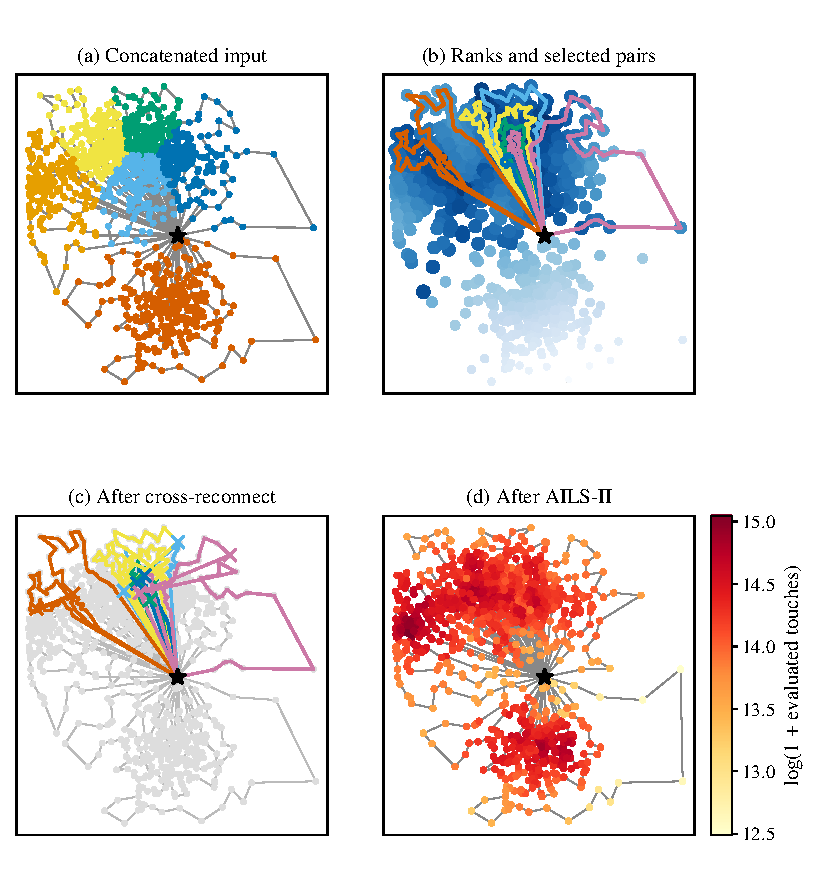
\includegraphics{figures/bgails_mechanism.pdf}
\caption{One BG-AILS call on XL-n1281-k29 (seed 101, $T = 60$\,s). Colorbar applies to panel~(d) only.}
\label{fig:bgails-mechanism}
\end{figure}

\begin{table}[H]
\centering
\caption{BG-AILS Parameters and Their Defaults.}
\label{tab:bg-ails-params}
\begin{tabular}{@{}p{3.3cm}p{1.7cm}p{7.3cm}@{}}
\toprule
Parameter & Default & Role \\
\midrule
Boundary threshold $\tau$ & 0.5 & Gates boundary ranks (Eq.~\ref{eq:bg-ails-threshold}); ranks at or below $\tau$ are zeroed. \\
Small-cluster cap $\sigma$ & 20 customers & Clusters below this size receive a boost in Eq.~\ref{eq:bg-ails-weighted}. \\
Small-cluster boost $\alpha$ & 0.5 & Maximum boost factor $1 + \alpha$, approached as cluster size $\to 0$. \\
Chain-count mode & $k$ & Number of cross-reconnect chains per call ($k - 1$ also implemented). \\
Pair selection & greedy & Deterministic arg-max vs.\ stochastic roulette-wheel route-pair draw. \\
Initial omega $\omega_0$ (\texttt{-initialOmega}) & 10 & Overrides AILS-II's own starting perturbation degree; see below. \\
Budget floor & 60\,s & Minimum AILS-II wall-clock limit regardless of the predicted model below. \\
Budget margin & 1.0 & Multiplier applied to the predicted decompose-route wall time. \\
\bottomrule
\end{tabular}
\end{table}

Table~\ref{tab:bg-ails-params} summarizes the parameters this stage introduces on top of stock AILS-II. Of these, only the initial-omega override reaches into AILS-II itself; every other AILS-II hyperparameter governing its own local search and diversification control (the parameters $d_{\min}$, $d_{\max}$, $\gamma$, and $\varphi$ of \citet{maximoHybridAdaptiveIterated2021}) is left at AILS-II's own defaults. Overriding $\omega$ to 10 against AILS-II's own starting value of roughly 30 lowers rather than raises the solver's internal perturbation degree: BG-AILS has already displaced customers across subcluster boundaries with its own cross-reconnect chain before AILS-II starts, so the pass that follows is asked to intensify around that disruption rather than to add more of its own. The remaining parameters -- the boundary threshold, the small-cluster cap and boost, the chain-count mode, and the pair-selection rule -- are new and govern only the Python-side perturbation step described above.

The key difference between BG-AILS and a plain AILS-II improvement pass is therefore not the solver itself but this focus on boundary regions, imposed both by the perturbation step and by the short wall-clock budget BG-AILS is given. That budget follows neither the fixed per-customer rate used for subcluster solving (Section~\ref{sec:fra-routing}) nor a plain function of instance size, but a fitted model of the surrounding decompose-route stage's own wall-clock time,
\begin{align}
\text{budget} &= \max\bigl(60\text{s},\ 1.0 \times \widehat{T}_{\mathrm{DR}}\bigr), \label{eq:bg-ails-budget}\\
\widehat{T}_{\mathrm{DR}} &= 0.976 \times n_{\mathrm{waves}}^{-0.180} \times \sum_{\text{waves}} \max(\text{per-cluster budgets in wave}), \label{eq:bg-ails-dr-wall}
\end{align}
refit on 835 post-strip pilot DRI iterations, where waves pack the current iteration's per-subcluster solver budgets (Section~\ref{sec:fra-routing}) into the granted DRI worker count in partition-submit order. This choice is deliberate: DRISPI can run BG-AILS in an asynchronous mode where a dedicated worker process perturbs and improves the current iteration's solution while the main process moves straight on to decomposing and routing the next iteration, with a single-slot handoff bounding the resulting lag to exactly one iteration. Sizing the BG-AILS budget after the very decompose-route stage it overlaps with is what keeps that overlap efficient rather than leaving either side idle; Section~\ref{sec:fra-pipeline} covers the resulting core split and this asynchronous handoff in full. By default, however, BG-AILS instead runs synchronously within the DRI iteration, still under the same Equation~\ref{eq:bg-ails-budget} budget.

Under this comparatively short wall-clock budget, BG-AILS should outperform an unguided AILS-II pass over the same combined solution, because the unguided pass spends an unknown and likely large share of that budget searching subcluster interiors the decomposition had already solved well. We tested this on all 100 XL instances (Section~\ref{sec:stu-dataset}) at three checkpointed decompose-route solutions each, all arms forked from the same checkpoint: a stock AILS-II pass at the solver's own defaults, a blind control that applies one cross-reconnect per subcluster to uniformly drawn route pairs, and BG-AILS in its deployed configuration (without-replacement first-route selection and a first local-search pass restricted to customers above $\tau$), the control and BG-AILS at $\omega = 10$. Every arm receives the same AILS-II budget, the checkpoint's own Equation~\ref{eq:bg-ails-budget} value; the Python-side perturbation of the two perturbing arms is a surplus on top of it, a median 0.28\% of that budget for BG-AILS and 0.010\% for the control. The checkpoints are generated under one pinned decomposition configuration, vertex K-Medoids, with HAOS, the route pool, and SC/SP out of the loop, so what is compared is one improvement stage against another on identical input, not two full runs.

BG-AILS statistically significantly outperforms both baselines (paired Wilcoxon signed-rank tests, alternative greater, Holm-corrected in a family of two). It improves on the stock AILS-II pass by 0.056~pp of cost improvement over the input solution (Hodges--Lehmann paired difference, 95\% CI $[0.049, 0.063]$, Holm-corrected $p = 7.0 \times 10^{-11}$, ahead on 85 of 100 instances) and on the blind control by 0.058~pp (95\% CI $[0.052, 0.065]$, Holm-corrected $p = 2.7 \times 10^{-12}$, ahead on 89 of 100). The AILS-II comparison is the practical one and carries the perturbation together with the $\omega$ override as the package the framework deploys. The control comparison holds $\omega$ and chain length fixed and isolates the boundary guidance itself. The paired difference between the control and stock AILS-II is consistent with zero (Hodges--Lehmann $-0.004$~pp, 95\% CI $[-0.011, 0.002]$), so the gain is not explained by perturbing the concatenated solution at all. Figure~\ref{fig:bgails-comparison} shows the arm means and the paired differences behind those tests.

\begin{figure}[H]
\centering
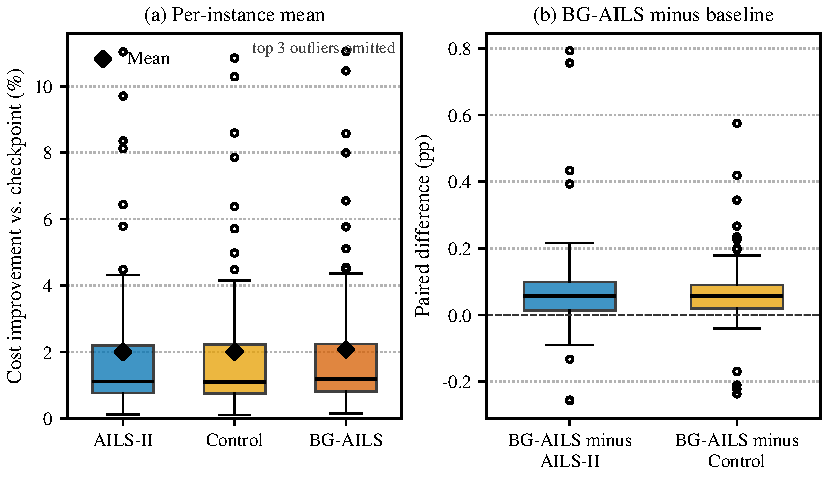
\includegraphics{figures/bgails_comparison.pdf}
\caption{Per-instance mean cost improvement (a) and paired BG-AILS differences (b). Top three outliers omitted in~(a).}
\label{fig:bgails-comparison}
\end{figure}

Three limits apply. The comparison is one DRI iteration, so it says nothing about what these routes are worth once the pool recombines them. It uses one pinned decomposition configuration, under which the clustering and the boundary metric read the same dissimilarity matrix, as they do for three of the eight deployed clustering methods but not for the five that cluster on raw coordinates or route centroids. The touch counts in Figure~\ref{fig:bgails-mechanism}(d) come from a separate, identically configured instrumented run rather than from the runs the costs above are measured on.

BG-AILS closes the DRI loop: its output routes are contributed to the route pool like every other stage's output (Section~\ref{sec:fra-sp}), and the next iteration begins with a fresh HAOS draw over the decomposition and routing levels (Section~\ref{sec:fra-haos}). Periodically, rather than continuing the DRI loop for another iteration, DRISPI instead steps back and recombines the pool accumulated across many such iterations through set covering or set partitioning, the subject of the next section.

\section{Route Pool and Set Partitioning}\label{sec:fra-sp}
% NOTE(citations-added-this-pass, not yet verified by the author): the following
% keys are new to bibliography/literature.bib as of this draft and should be
% checked for relevance and correctness before the next build:
% rochatProbabilisticDiversificationIntensification1995, balinskiIntegerProgramDelivery1964,
% garfinkelSetPartitioningProblemSetCovering1969, jaccardDistributionFloreAlpine1901,
% cavaliereIntegratedLocalsearchSetpartitioning2022, hybridizing_jourdan_2009,
% lubbeckeSelectedTopicsColumn2005.

% ensure the abbreviations SC/SP are introduced either here or before

Periodically, DRISPI steps back from the current incumbent and recombines every route accumulated so far into one new candidate solution, using set covering or set partitioning (SC/SP) as the recombination model. Alternating a metaheuristic with an exact set-partitioning solve in this way is an established matheuristic pattern \citep{hybridizing_jourdan_2009}. \citet{cavaliereIntegratedLocalsearchSetpartitioning2022} apply essentially this pairing to large-scale \gls{cvrp} instances directly, by alternating LKH-3 local search with a restricted set-partitioning solve. Doing so only pays off if a shared memory of routes exists for it to recombine, so this section first describes that memory, the route pool, before turning to the SP and SC models themselves and the hyperparameter that decides between them.

The route pool stores one entry per distinct customer set $C_r \subseteq C$, where $C$ is the customer set of the instance (Section~\ref{sec:lit-problem}), keyed by the frozen customer set rather than by the ordered sequence of customers a route visits them in: two routes serving the same customers in a different order, or at a different cost, are treated as the same column, and the cheaper of the two overwrites the other. This column-oriented memory, populated online during the DRI loop and periodically recombined through a partitioning model, follows the adaptive-memory principle of \citet{rochatProbabilisticDiversificationIntensification1995}, who introduce the route pool and its set-partitioning recombination for vehicle routing.

Two pathways feed the pool every iteration, both through the same contribute-before-adopt rule: a candidate solution is added to the pool before the pipeline decides whether to adopt it as the new incumbent, so a losing candidate still leaves its routes behind for later reuse. The DRI loop feeds the pool at least twice per iteration, once from its decompose-route stage (Section~\ref{sec:fra-routing}) and once from the following improvement stage (BG-AILS (Section~\ref{sec:fra-bg-ails})). The SC/SP step covered in this section feeds the pool only indirectly. Solving SC or SP selects among the customer sets already in the pool and creates no new ones, so its own output adds nothing. The post-SC/SP-improvement pass that polishes its result (Section~\ref{sec:fra-improve}) is what can move customers between routes and through that generate new columns. Every contributed route carries a tag recording the full HAOS selection that produced it, that is, k, the demand weight, the paradigm, the method, and the solver, with a separate flag marking routes from the post-SC/SP polish; the tag survives even once HAOS has moved on to a different selection, which is what later lets reward attribution and pool inspection trace a route back to its origin. Whenever a candidate is adopted as the new incumbent, its routes, already in the pool by the rule above, are marked elite; elite routes are exempt from eviction, so the pool never loses the one partition it is guaranteed to already have, namely the incumbent's own.
% decide if I want to cut the sentence about HAOS or if this is a repitition to 4.1

Every SC/SP solve also updates two running scores on each pool entry: A quality and a diversity score. The quality score represents a column's usefulness for the solver during the SC/SP solve. Therefore, an entry never touched by a solve carries no quality score yet. The diversity score is the mean Jaccard distance \citep{jaccardDistributionFloreAlpine1901} between a route's customer set and every other pool entry's customer set,
\begin{equation}
\bar{J}(r) = \frac{1}{|R| - 1} \sum_{r' \in R \setminus \{r\}} \frac{|C_r \triangle C_{r'}|}{|C_r \cup C_{r'}|},
\label{eq:route-diversity}
\end{equation}
where $R$ is the pool at the time of the update, recomputed for every entry whenever any solve happens. New quality or diversity scores are appended to a three-value window, from which final scores are read as the mean of their respective window. This ensures that single unusually high or low values do not dominate a route's standing.

The route pool has a maximum size (10,000 columns by default), to keep the computational complexity from blowing up. We therefore establish an eviction policy that ranks the non-elite entries on both scores and combines the ranks into one fitness value. Among the entries that have been scored at least once, ascending order by mean quality score gives rank one to the weakest route and the highest rank to the strongest; independently, ascending order by mean diversity score gives rank one to the most redundant route and the highest rank to the most unique. Writing $\rho_q(r)$ and $\rho_d(r)$ for these two ranks, fitness is $\Phi(r) = \rho_q(r) + w_d \cdot \rho_d(r)$, with the diversity weight $w_d$ (0.5 by default) controlling how much redundancy counts against a route relative to raw quality. The entries with the lowest $\Phi(r)$ are evicted first. Because both terms grow toward the same end of their respective orderings, a route that the LP relies on heavily but that is also nearly identical to several other pool entries can rank as a stronger eviction candidate than a weak but singular one, because redundancy drives the diversity term up regardless of quality. The eviction policy only triggers once the pool exceeds its maximum size and then only removes the overflow amount. Unscored entries are evicted only if the overflow cannot be covered by scored, non-elite entries alone. Elite entries are categorically exempt from eviction.

The recombination model itself treats the pool as a column set. Let $R$ be the set of routes currently in the pool, $c_r$ the cost of route $r \in R$, that is, the Euclidean depot-customers-depot round trip over the travel costs of Section~\ref{sec:lit-problem}, and $x_r \in \{0, 1\}$ a decision variable selecting route $r$. Set partitioning, in the formulation \citet{balinskiIntegerProgramDelivery1964} introduce for exactly this delivery-routing setting, reads
\begin{align}
\text{min} \quad & \sum_{\mathclap{r \in R}} c_r x_r \label{eq:sp-obj}\\
\text{s.t.} \quad & \sum_{\mathclap{r \in R:\, i \in C_r}} x_r = 1, && \forall i \in C \label{eq:sp-partition}\\
& x_r \in \{0, 1\}, && \forall r \in R. \label{eq:sp-binary}
\end{align}
Solving Equations~\ref{eq:sp-obj}--\ref{eq:sp-binary} recombines route fragments that have never been jointly considered, for example because they may have entered the pool from different subclusters, different HAOS selections, or different iterations, into one coherent solution that still covers every customer exactly once. This is the sense in which SP looks across the boundaries any individual DRI iteration's decomposition imposes, something no individual subcluster solve or BG-AILS perturbation can do on its own.

DRISPI builds this model once in Gurobi\footnote{\url{https://www.gurobi.com}} and solves it twice. It first relaxes Equation~\ref{eq:sp-binary} to the continuous $x_r \in [0, 1]$ and solves the resulting linear program. This LP relaxation allows the solver to assign fractional weights rather than the binary ones to each route, making it significantly easier and faster to solve. The resulting fractional weights are then utilized as the quality scores fed back into the route pool above, so every SC/SP solve doubles as a scoring pass over the pool regardless of what it ultimately selects. This follows the same spirit in which column-generation approaches read pricing information out of LP duals \citep{lubbeckeSelectedTopicsColumn2005}, even though DRISPI's route pool is populated by heuristic solves rather than a pricing subproblem. For the second solve, the variables are then switched to binary, warm-started from the LP solution, and re-optimized as a mixed-integer program under a wall-clock time limit and a relative optimality gap (720 seconds and 0.025\% by default). A wallclock time limit is required to cut off the search with a good, if not provably optimal, solution rather than run to completion.

The equality constraint of Equation~\ref{eq:sp-partition} is only a meaningful choice if the pool offers more than one real alternative for most customers. A pool still dominated by a single incumbent partition would just reproduce it again and again under SP. DRISPI therefore checks, before every SC/SP trigger, whether every customer in the instance is covered by at least a fixed minimum number of pool routes (five by default). Only when that holds does SP run. Otherwise DRISPI falls back to the less constrained set covering (SC), the inequality-constrained relaxation of the same formulation \citep{garfinkelSetPartitioningProblemSetCovering1969}, whose formal problem statement and LP relaxation are given in Appendix~\ref{app:set-covering}. SC only requires every customer to be covered at least once rather than exactly once, a condition the pool always satisfies, because the elite routes described above are never evicted and already form a feasible partition on their own. This is also why the fallback is safe and not merely convenient: SP is never blocked by infeasibility, only by a pool that has not yet accumulated enough alternatives, and SC exists to give the SC/SP step something well defined and always solvable to run on every scheduled trigger, warmup aside, no matter how much the pool has matured. The price of that permissiveness is that SC's selected routes can overlap on a customer, meaning a customer can be visited by more than a single route and therefore more than exactly once. Since this would violate our problem statement formulated in Section~\ref{chapter:problem}, a savings-based deduplication heuristic then removes each duplicated customer from every selected route except the one where removing it would save the least cost, restoring a feasible partition.

A solved partitioning problem will pair routes into a new candidate solution which haven't been evaluated together before. And while search heuristics have been employed in identifying the routes used, the resulting new set of routes has not been polished by evaluating for example inter-route moves amongst each other. To do just that the SC/SP step is combined with a standard-AILS pass (Section~\ref{sec:fra-improve}) to improve the partitioning result even further if possible.

\section{Improvement}\label{sec:fra-improve}
Once SC/SP (Section~\ref{sec:fra-sp}) recombines the route pool into one partition, DRISPI runs one further pass over it using AILS-II as solver, seeded only with that partition as an initial solution. Unlike in BG-AILS (Section~\ref{sec:fra-bg-ails}), this step focuses less on perturbation but rather refinement by local search. This standard improvement step also allows the solver to touch all routes instead of biasing moves towards certain neighborhoods. The pass runs under its own wall-clock budget (360 seconds by default) on the same core reservation as the SC/SP solve that precedes it; Section~\ref{sec:fra-pipeline} covers how exactly a parallel architecture of DRISPI looks.

The refined routes feed back into the route pool exactly like every other stage's output (see Section~\ref{sec:fra-sp}): a route whose customer set matches one SC/SP already selected keeps that route's existing tag, while a route AILS-II creates by moving customers between routes is added as new, tagged as an improvement route rather than credited to a HAOS selection of its own.

This is also where the deferred half of HAOS's reward system (Section~\ref{sec:fra-haos}) closes. The pass's outcome, a new best, an improvement over the previous iteration without beating the incumbent, or neither, is scored through the deferred branch of HAOS's reward function and credited not to the current iteration's own draw but to every distinct HAOS tag the routes SC/SP selected already carried, that is, to whichever earlier decompose-route or BG-AILS draws produced those specific routes, regardless of how many iterations ago that was. Improvement-route tags are excluded from this credit, since AILS-II created them without any HAOS draw of their own to reward.

\section{Pipeline Orchestration}\label{sec:fra-pipeline}
The preceding sections describe HAOS, decomposition, routing, BG-AILS, the route pool and SC/SP, and the post-SC/SP improvement pass as if the DRI loop executed them one after another, the sequential picture Figure~\ref{fig:dri-overview} shows. DRISPI instead runs three of these stages as separate worker groups sharing one CPU allocation, so that a DRI iteration and the BG-AILS or SC/SP work left over from an earlier one can occupy the same wall-clock interval instead of queuing behind each other. This section describes that parallelized pipeline.

DRISPI splits its CPU allocation into three disjoint worker groups: $\mathrm{dri}$ cores for the subcluster routing pool of Section~\ref{sec:fra-routing}, $\mathrm{bg}$ cores for the BG-AILS worker of Section~\ref{sec:fra-bg-ails}, and $\mathrm{sp}$ cores for the SC/SP and post-SC/SP improvement worker of Sections~\ref{sec:fra-sp} and~\ref{sec:fra-improve}. The deployed split for the 100-instance campaign of Chapter~\ref{chapter:study} is 6+1+1 inside each 8-core Docker container (Section~\ref{sec:stu-implementation}), the \texttt{cores} block of \texttt{configs/final\_benchmark.yaml}; the split is a configuration value, not a fixed architectural constant, and a deployment with more cores per container widens $\mathrm{dri}$ rather than the other two groups, since subcluster routing is the stage with an unbounded number of independent jobs per iteration.

BG-AILS and SC/SP each support a synchronous and an asynchronous mode, and the two modes differ in the same way for both stages: synchronously, the stage runs inline inside the current DRI iteration and the loop waits for it; asynchronously, a long-lived worker process owns the stage's reserved cores across iterations, and the main loop dispatches a job to it without waiting for the result. DRISPI's own configuration default is synchronous for both stages, matching the sequential description of Section~\ref{sec:fra-bg-ails} and Section~\ref{sec:fra-sp}; the asynchronous mode is implemented for both and is what \texttt{configs/final\_benchmark.yaml} enables for the campaign behind Chapter~\ref{chapter:study}, since only the asynchronous mode lets the $\mathrm{bg}$ and $\mathrm{sp}$ cores do anything while the $\mathrm{dri}$ cores are busy on the next iteration.

The BG-AILS worker uses a single-slot handoff: at most one BG-AILS job is ever in flight. The main loop dispatches the current iteration's combined decompose-route solution to the worker and moves straight on to decomposing and routing the next iteration on the $\mathrm{dri}$ cores; at the start of the iteration after that, before drawing a new HAOS configuration, the loop blocks until the worker returns, drains the result, and only then dispatches the next job. This bounds the resulting lag to exactly one iteration by construction, never more, because the loop will not dispatch a second job while the first is outstanding. Equation~\ref{eq:bg-ails-budget} sizes the BG-AILS wall-clock budget against a fitted model of the very decompose-route stage it overlaps with, rather than against instance size directly, precisely because that overlap is the point of running BG-AILS asynchronously: a budget much shorter than the next decompose-route stage would leave the $\mathrm{bg}$ core idle before the handoff, and a budget much longer would leave the $\mathrm{dri}$ cores waiting on a BG-AILS job that already had the next iteration's input ready.

The SC/SP worker instead uses a skip overlap policy rather than a blocking handoff. When a scheduled SC/SP trigger comes due, either every \texttt{sp\_interval} iterations or, as configured for the campaign, every 20 minutes of wall-clock time, DRISPI dispatches a snapshot of the route pool and the current incumbent to the SP worker only if that worker is not already busy with a previous job; if it is, the trigger is skipped outright rather than queued, and the pipeline tries again at the next scheduled trigger. This is why the SC/SP branch never stalls the $\mathrm{dri}$ or $\mathrm{bg}$ workers: a slow SP solve, the 720-second time limit of Section~\ref{sec:fra-sp} is a ceiling, not a typical duration, can only cause a later trigger to be skipped, never a delay elsewhere in the loop. The SP worker owns both the SC/SP solve and the post-SC/SP improvement pass of Section~\ref{sec:fra-improve} for a given job, running them one after another on the same $\mathrm{sp}$-core reservation before the result becomes available for the main loop to drain.

Figure~\ref{fig:pipeline-swimlane} shows this overlap across two consecutive iterations, one lane per worker group: the $\mathrm{dri}$ lane occupied by decomposition and routing in every iteration, the $\mathrm{bg}$ lane running one iteration behind it under the single-slot handoff, and the $\mathrm{sp}$ lane occupied only when a trigger fires, spanning several $\mathrm{dri}$ iterations without blocking them.

\begin{figure}[H]
\centering
\todo{FIGURE: swimlane diagram over wall-clock time, one horizontal lane each
for the dri, bg, and sp worker groups, spanning two consecutive DRI
iterations. dri lane: back-to-back decompose+route blocks, one per
iteration. bg lane: one perturb+improve block per iteration, offset to
start when the dri block of the same iteration ends and to finish before
the dri block of the iteration after next begins (single-slot handoff,
one-iteration lag). sp lane: mostly idle, with one long solve+improve
block spanning multiple dri iterations, triggered every 20 minutes of
wall-clock time (final\_benchmark.yaml), with an arrow marking a
would-be trigger that is skipped because the previous sp block is still
running. Requires the actual per-stage wall-clock durations from a
representative run; not fabricated here.}
\caption{Core allocation and cross-iteration overlap in DRISPI's parallelized pipeline.}
\label{fig:pipeline-swimlane}
\end{figure}

Algorithm~\ref{alg:pipeline} gives the resulting control loop from the main process's perspective, in the asynchronous form both stages run under for the campaign of Chapter~\ref{chapter:study}; the synchronous default replaces every dispatch of a BG-AILS or SC/SP job with an inline call that blocks the loop until that job returns, collapsing the loop back to Figure~\ref{fig:dri-overview}'s sequential picture.

\begin{algorithm}[H]
\DontPrintSemicolon
\LinesNumbered
\SetKwInOut{Input}{Input}
\SetKwInOut{Output}{Output}
\Input{instance; HAOS wheels (Algorithm~\ref{alg:haos}); $\mathrm{dri}$/BG/SP workers; route pool $R \gets \emptyset$; incumbent $S^\star \gets \mathrm{None}$; limits $\Gamma, \Pi$}
\Output{incumbent $S^\star$ at termination}
$i \gets 0$\;
\While{elapsed time $< \Gamma$ and iterations since improvement $< \Pi$}{
  \If{$i > 0$ and the BG worker is busy}{
    join (blocking): drain $S_{\mathrm{bg}}^{(i-1)}$\;
    contribute its routes to $R$; adopt as $S^\star$ if improving; credit immediate reward\;
  }
  \If{the SP worker has a completed job}{
    drain (non-blocking): contribute its routes to $R$; adopt as $S^\star$ if improving; credit deferred reward per tag; free the SP worker\;
  }
  $(k, \lambda_q, \mathrm{paradigm}, \mathrm{method}, \mathrm{solver}) \gets$ HAOS-Draw() \tcp*{Algorithm~\ref{alg:haos}}
  partition $\gets$ decompose $k$ subclusters under $(\lambda_q, \mathrm{paradigm}, \mathrm{method})$\;
  dispatch one routing job per subcluster to the $\mathrm{dri}$ pool\;
  join: collect all $k$ subcluster solutions\;
  $S_{\mathrm{dr}}^{(i)} \gets$ concatenate them\;
  contribute $S_{\mathrm{dr}}^{(i)}$ routes to $R$; adopt as $S^\star$ if improving; credit immediate reward\;
  dispatch $(S_{\mathrm{dr}}^{(i)}, \mathrm{partition})$ to the BG worker \tcp*{single-slot handoff}
  \If{SC/SP is scheduled at iteration $i$}{
    \eIf{the SP worker is busy}{
      skip this trigger \tcp*{overlap: skip, not queue}
    }{
      dispatch a snapshot of $(R, S^\star)$ to the SP worker\;
      \lIf{coverage $\geq$ minimum in the snapshot}{solve SP}
      \lElse{solve SC; deduplicate}
      run the post-SC/SP improvement pass on the result\;
    }
  }
  $i \gets i + 1$\;
}
\Return{$S^\star$}
\caption{DRISPI: parallelized pipeline control loop (asynchronous BG-AILS and SC/SP)}
\label{alg:pipeline}
\end{algorithm}

Lines 15-22 are the scheduled SC/SP branch: the coverage check and the resulting SP-or-SC choice (lines 20-21) and the post-SC/SP improvement pass (line 22) are the same procedure Section~\ref{sec:fra-sp} and Section~\ref{sec:fra-improve} describe, dispatched as one job rather than run inline; line 17 is the skip that keeps a busy SP worker from ever blocking the loop above it. Lines 3-5 are the asynchronous BG-AILS handoff on the reading side: the join only happens once the worker is already busy from a previous dispatch (line 3), so the first iteration never blocks, and every iteration after that blocks on exactly one prior job (line 4) before line 14 hands the worker a new one, which is what keeps the BG lag fixed at one iteration regardless of how the rest of the loop's timing drifts.

Lines 5, 7, and 13 are the three points where a candidate's routes enter $R$ before the pipeline decides whether to adopt it as $S^\star$, one per worker group, BG, SP, and DRI respectively, the contribute-before-adopt rule of Section~\ref{sec:fra-sp} applied uniformly across all three: a candidate that does not become the new incumbent still leaves its routes in the pool for a later SC/SP call to draw on. The post-SC/SP improvement pass on lines 19-22 produces a fourth candidate, but because that job runs asynchronously, its contribution and adopt check happen only when line 7 drains it in a later iteration, not inline within lines 15-22 themselves.